\tikzset{every node/.style={scale=0.8}}
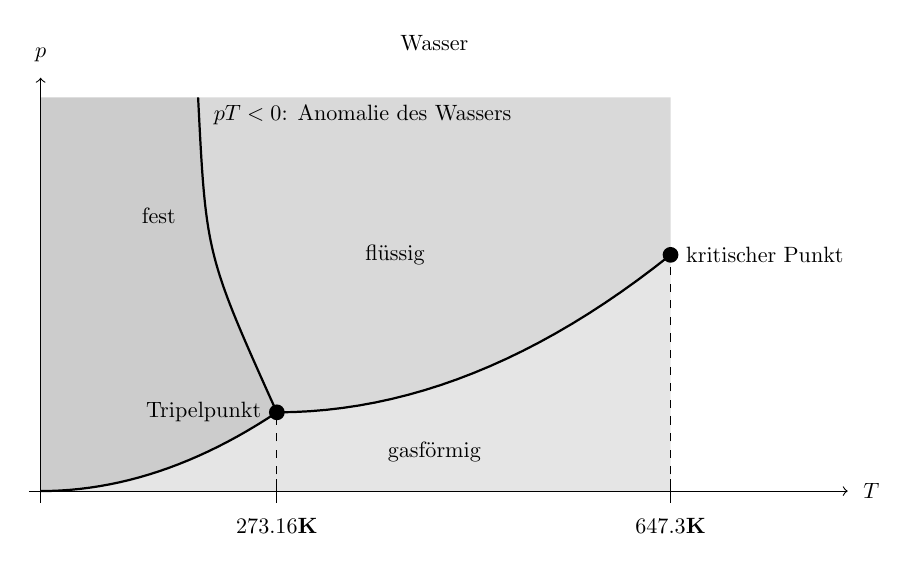
\begin{tikzpicture}[baseline=2.5cm]

  \fill[white!90!black,domain=0:3] (0,0) -- plot (\x,{(\x^2)/9}) -- (3,1) -- (3,0) -- cycle;
  \fill[white!90!black,domain=3:8] (3,0) -- (3,1) -- plot (\x,{2*((\x-3)^2)/25+1}) -- (8,3) -- (8,0) -- cycle;

  \fill[white!80!black,domain=0:3] (0,0) -- plot (\x,{(\x^2)/9}) -- (3,1) .. controls (2.1,3) .. (2,5) -- (0,5) -- cycle;

  \fill[white!85!black,domain=3:8] (2,5) ..  controls (2.1,3) .. (3,1) -- plot (\x,{2*((\x-3)^2)/25+1}) -- (8,3) -- (8,5) -- cycle;

  \draw[->] (0,-0.15) to (0,5.25);
  \draw[->] (-0.15,0) to (10.25,0);
  \node[anchor=south] at (0,5.35) {$p$};
  \node[anchor=west] at (10.35,0) {$T$};

  \draw[thick,domain=0:3] plot (\x,{(\x^2)/9});
  \draw[thick,domain=3:8] plot (\x,{2*((\x-3)^2)/25+1});

  \draw[thick] (3,1) .. controls (2.1,3) .. (2,5);

  \draw (3,-0.15) to ++ (0,0.3);
  \draw[dashed] (3,0) to ++ (0,1);
  \node[anchor=north] at (3,-0.25) {$273.16\textbf{K}$};

  \draw (8,-0.15) to ++ (0,0.3);
  \draw[dashed] (8,0) to ++ (0,3);
  \node[anchor=north] at (8,-0.25) {$647.3\textbf{K}$};

  \node[anchor=south] at (5,5.5) {\uline{Wasser}};

  \fill[black] (3,1) circle (0.1);
  \fill[black] (8,3) circle (0.1);

  \node at (1.5,3.5) {fest};
  \node at (4.5,3) {flüssig};
  \node at (5,0.5) {gasförmig};

  \node[anchor=west] at (8.1,3) {kritischer Punkt};
  \node[anchor=east] at (2.9,1) {Tripelpunkt};

  \node[anchor=north west] at (2.1,5) {$\ddv{p}{T} < 0$: Anomalie des Wassers};

\end{tikzpicture}
